%!TEX root = memoria_duocode_interfaz.tex

En esta sección se muestra el funcionamiento de la aplicación web desde el punto de vista de un usuario.

\subsection{Lenguajes}
Al acceder al inicio de la web se nos muestran un par de listas con lenguajes de programación, donde podremos elegir cuál sabemos y cuál queremos aprender, en ningún caso será posible elegir la misma opción en ambos lados. En la parte superior se encuentra la barra de navegación que estará accesible en todo momento.

\begin{figure}[H]
\begin{center}
\makebox[\textwidth]{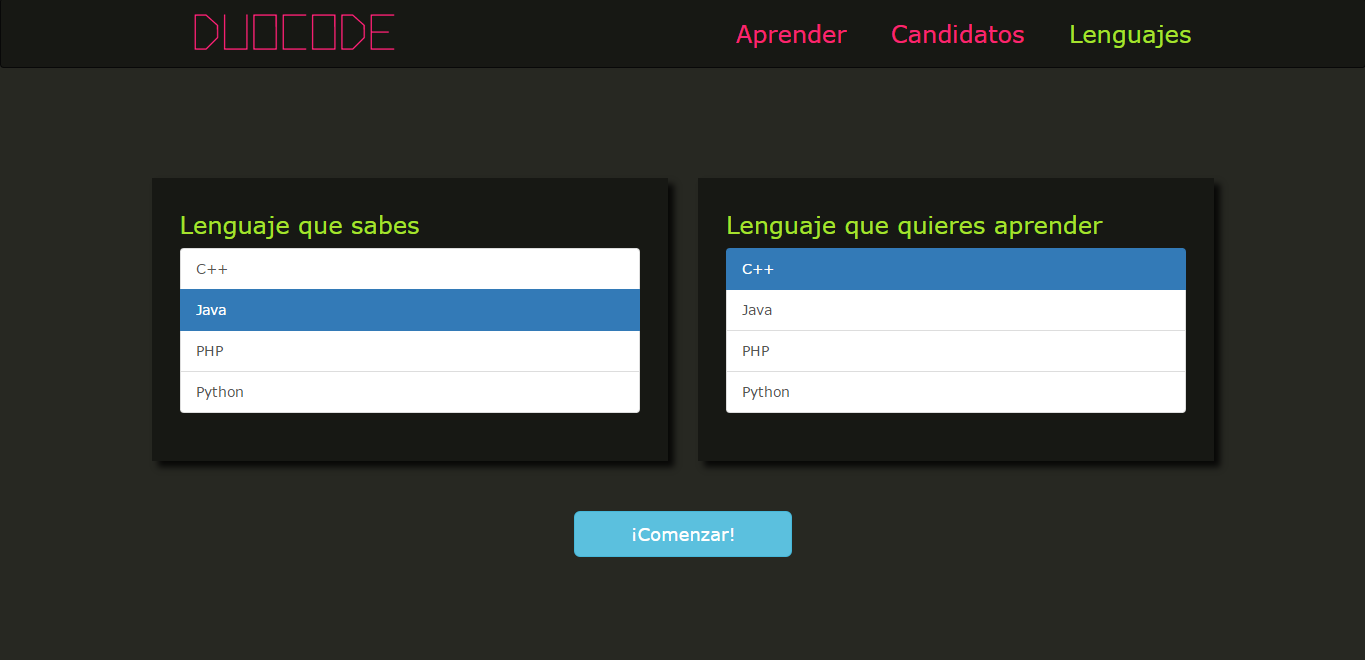
\includegraphics[scale=0.4]{images/lenguajes}}
\end{center}
\end{figure}

Una vez pulsado el botón de ``¡Comenzar!'', pasamos a la página de los temas.

\subsection{Temas}
En esta sección nos encontramos con dos partes diferenciadas. Por una parte, tenemos el login/información de usuario y por otra todos los temas disponibles con una breve explicación sobre estos.

\begin{figure}[H]
\begin{center}
\makebox[\textwidth]{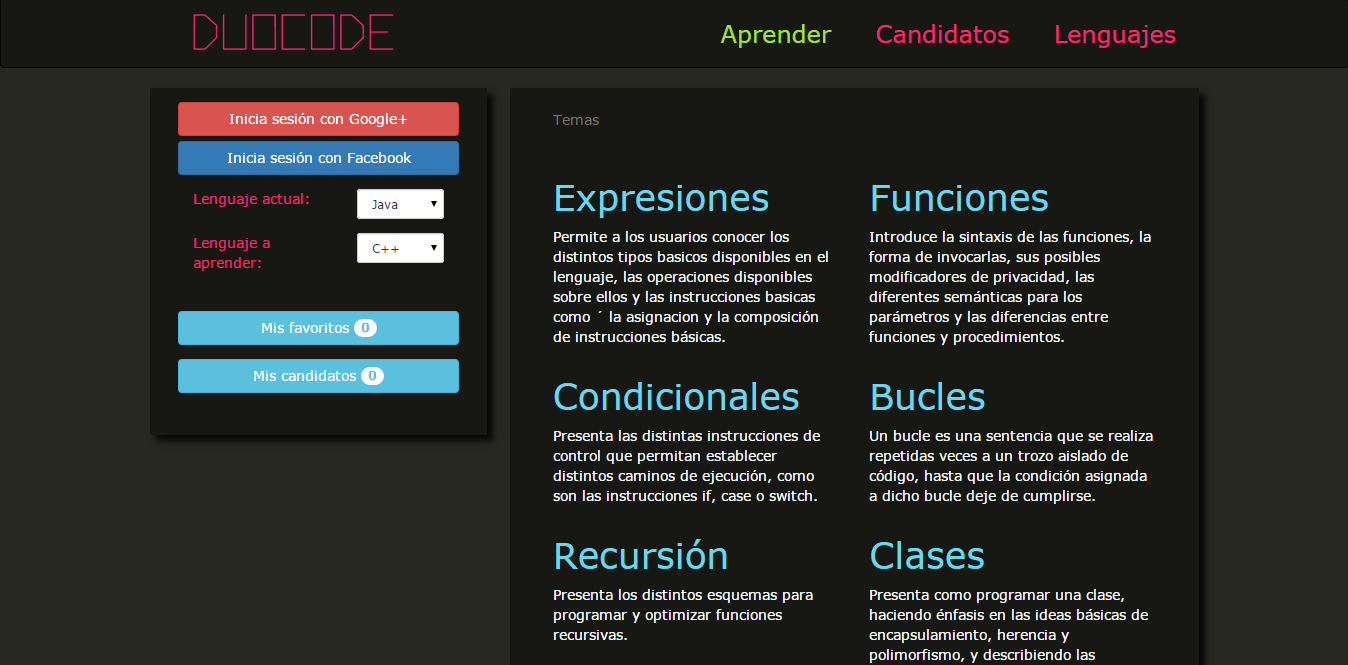
\includegraphics[scale=0.4]{images/temas}}
\end{center}
\end{figure}

Tenemos la posibilidad de iniciar sesión tanto con Google como con Facebook.

\begin{figure}[H]
\begin{center}
\makebox[\textwidth]{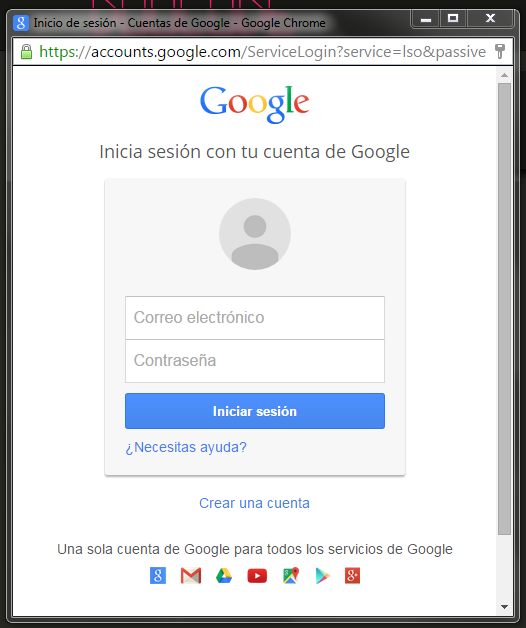
\includegraphics[scale=0.6]{images/Google}}
\end{center}
\end{figure}

\begin{figure}[H]
\begin{center}
\makebox[\textwidth]{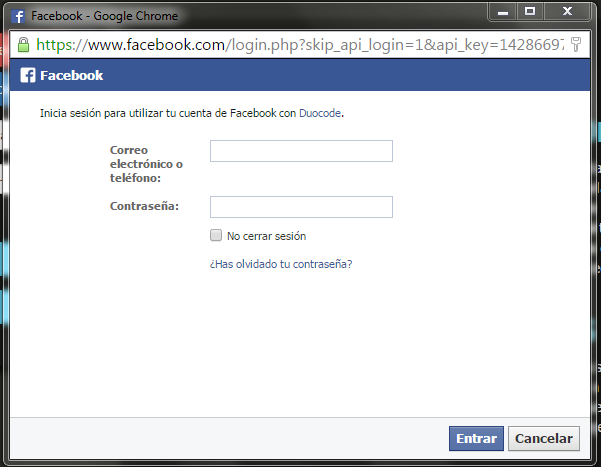
\includegraphics[scale=0.6]{images/Facebook}}
\end{center}
\end{figure}

En ambos casos se pedirá permiso al usuario para acceder a su información de perfil. Después de iniciar sesión, en la información de usuario aparecerá el nombre y la imagen de su perfil de red social, su puntuación total en DuoCode, los lenguajes seleccionados anteriormente, su número de ejercicios favoritos y candidatos enviados en la aplicación. 

\begin{figure}[H]
\begin{center}
\makebox[\textwidth]{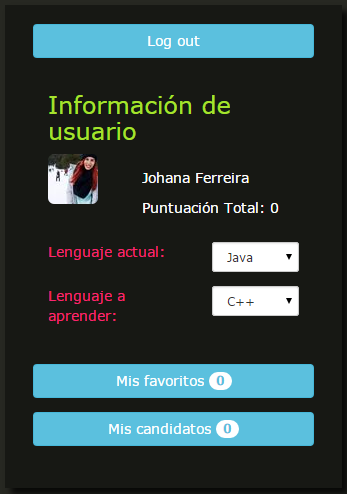
\includegraphics[scale=0.6]{images/usuario}}
\end{center}
\end{figure}

Una vez seleccionado un tema, pasamos a las lecciones.

\subsection{Lecciones}

Al seleccionar un tema accedemos a sus correspondientes lecciones, de las cuales podemos ver un pequeño resumen. Si el nombre de la lección aparece en blanco significa que esta es dependiente de otra, es decir, tienes que superar antes otra lección para poder acceder a esta.

\begin{figure}[H]
\begin{center}
\makebox[\textwidth]{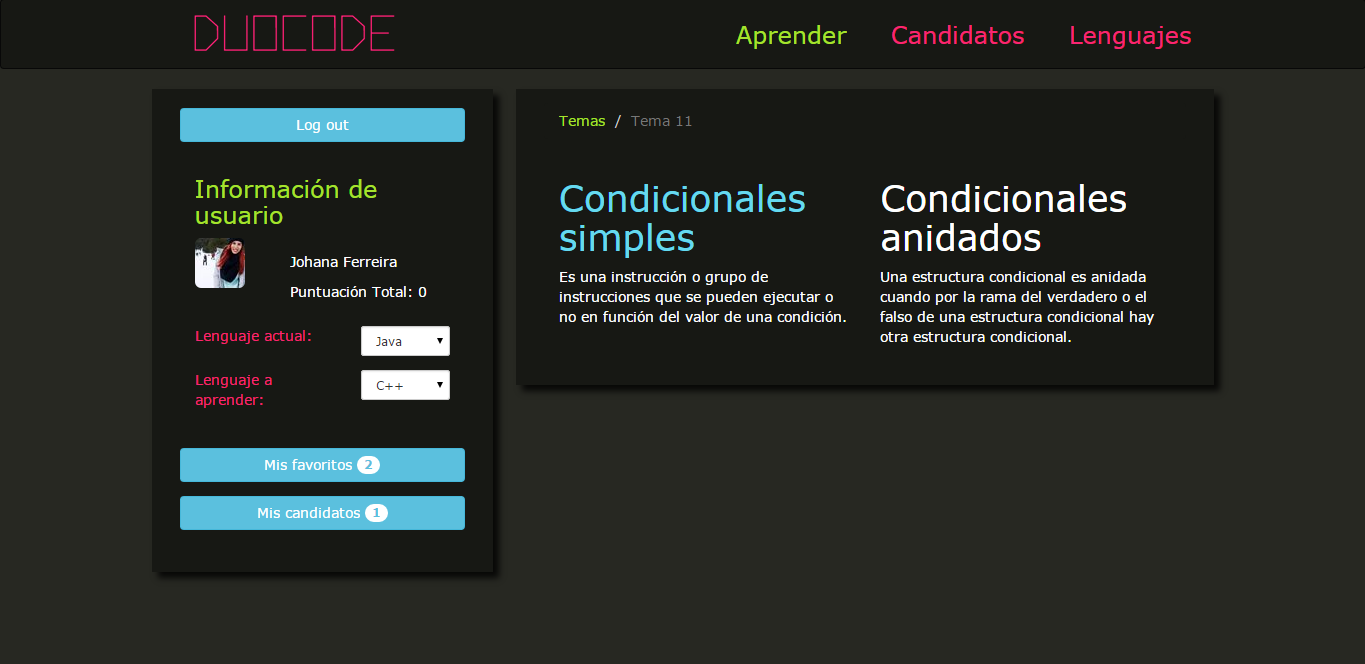
\includegraphics[scale=0.4]{images/lecciones}}
\end{center}
\end{figure}

Una vez seleccionada una lección, pasamos a los ejercicios.

\subsection{Ejercicios}

En esta parte lo primero que nos encontramos es un \textit{pop-up} con una explicación de la lección, al que se podrá acceder nuevamente a lo largo de esta. 

\begin{figure}[H]
\begin{center}
\makebox[\textwidth]{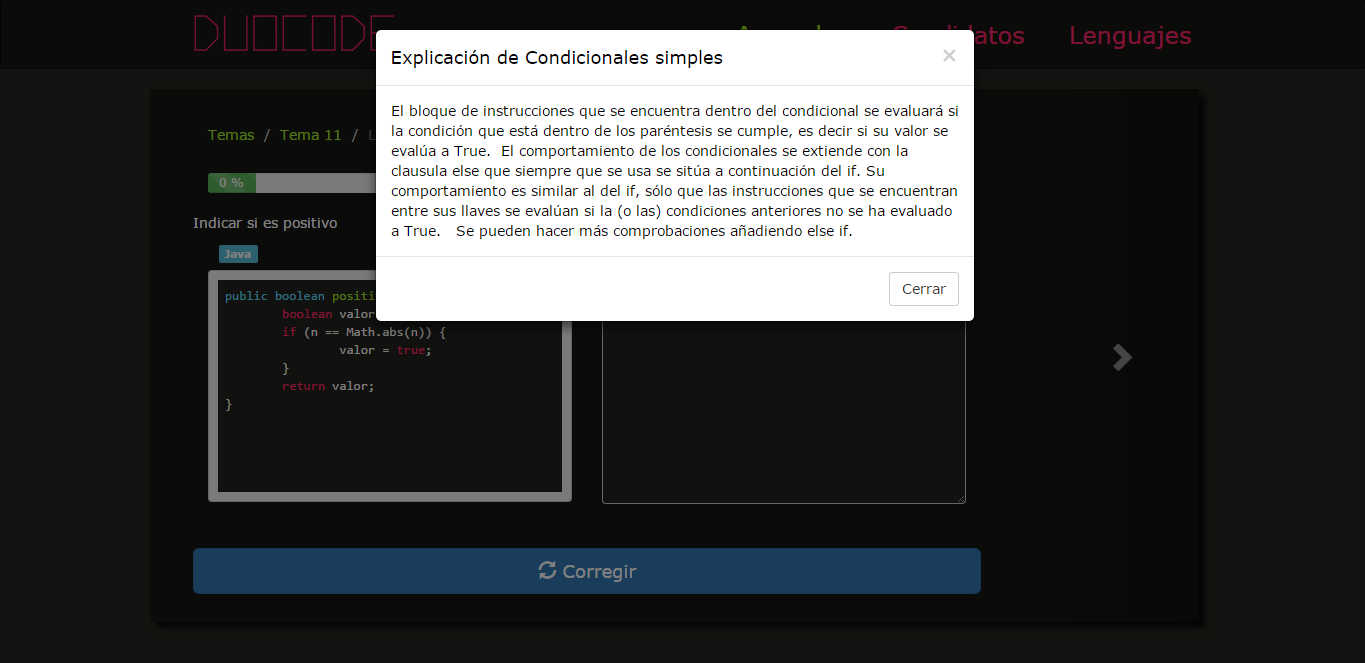
\includegraphics[scale=0.4]{images/popup}}
\end{center}
\end{figure}

Al cerrar el \textit{pop-up} empezamos con los ejercicios. En todo momento encontramos varios elementos en la parte superior: una barra en la que se indica el porcentaje que se ha completado de la lección, las vidas restantes, un botón para añadir a favorito el ejercicio actual y un botón de ayuda con el que se muestra el \textit{pop-up} del principio.

\vspace{1em}

Para cada ejercicio se muestra su título y dos cuadros de código, uno con el del enunciado del ejercicio y otro vacío que es donde el usuario tendrá que resolver el ejercicio.

\vspace{1em}

Por último está el botón de ``Corregir'' con el cual enviamos el ejercicio a ser corregido.

\begin{figure}[H]
\begin{center}
\makebox[\textwidth]{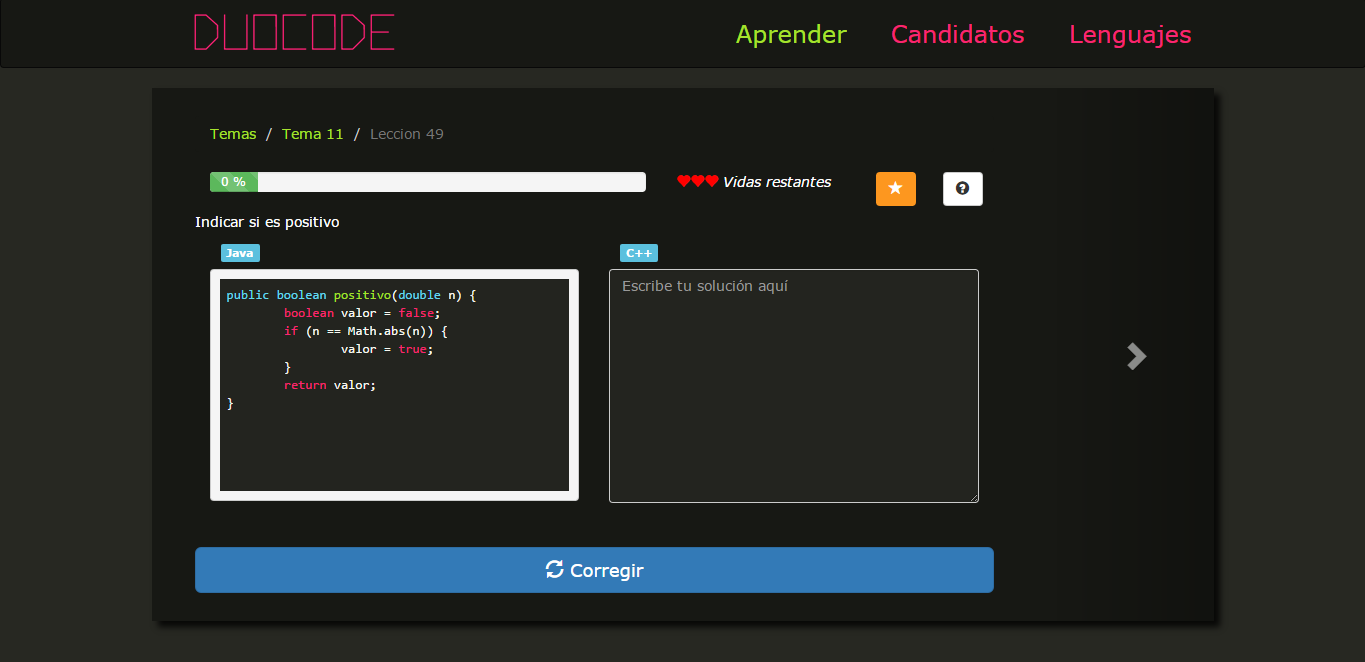
\includegraphics[scale=0.4]{images/ejercicio}}
\end{center}
\end{figure}

Después de corregir el ejercicio hay dos posibilidades:
\begin{itemize}
\item[•]Solución correcta: En este caso se muestra un mensaje con la puntuación obtenida.

\begin{figure}[H]
\begin{center}
\makebox[\textwidth]{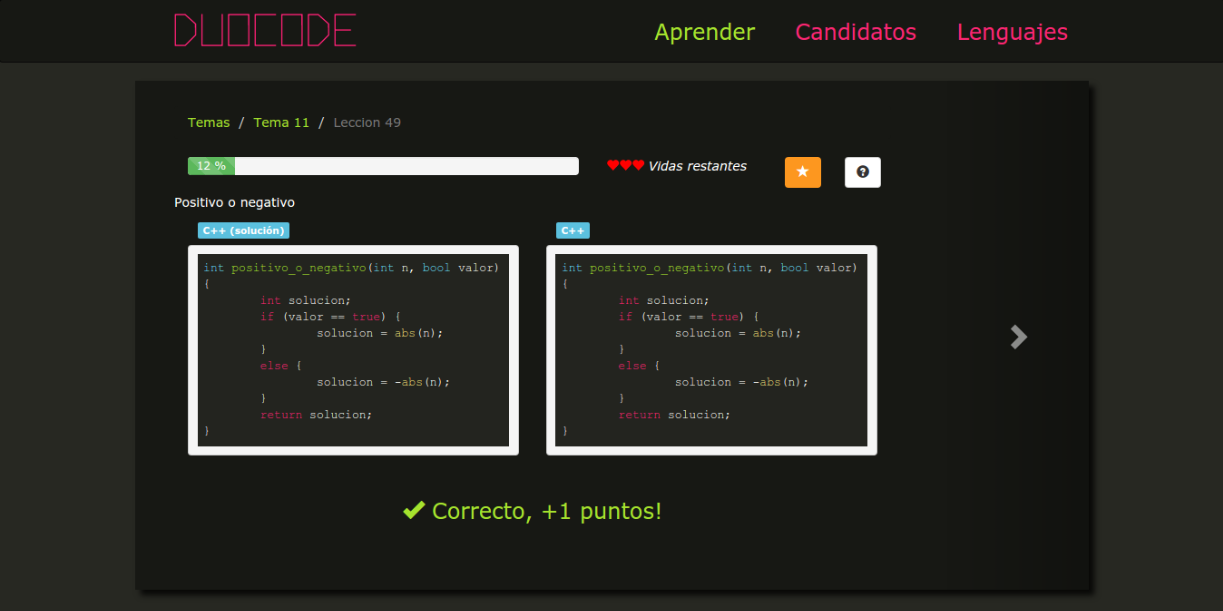
\includegraphics[scale=0.45]{images/ejercicioCorrecto}}
\end{center}
\end{figure}

\item[•]Solución incorrecta: En este caso se resta un corazón, se muestra un mensaje de incorrecto y la puntuación obtenida. Donde estaban anteriormente el código de enunciado y la solución del usuario ahora se muestra el enunciado y la solución correcta. También se da la posibilidad al usuario de enviar su ejercicio como candidato si piensa que la solución que dio era correcta; si el usuario no sabe qué son los candidatos se encuentra también un botón con un \textit{pop-up} explicativo.

\begin{figure}[H]
\begin{center}
\makebox[\textwidth]{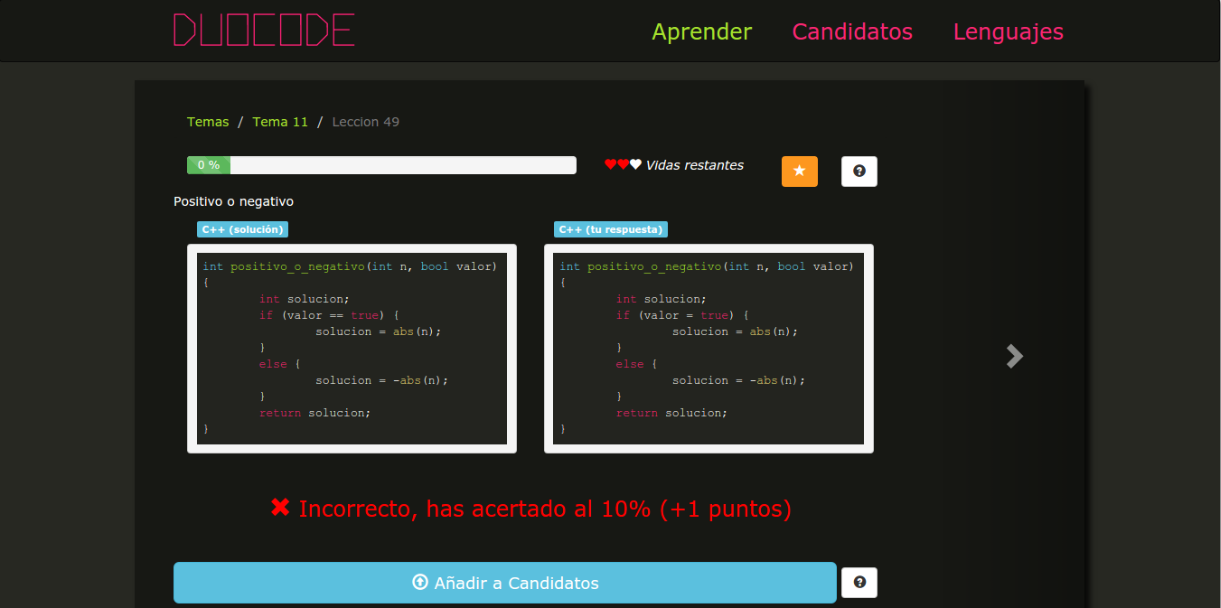
\includegraphics[scale=0.45]{images/ejercicioIncorrecto}}
\end{center}
\end{figure}

\begin{figure}[H]
\begin{center}
\makebox[\textwidth]{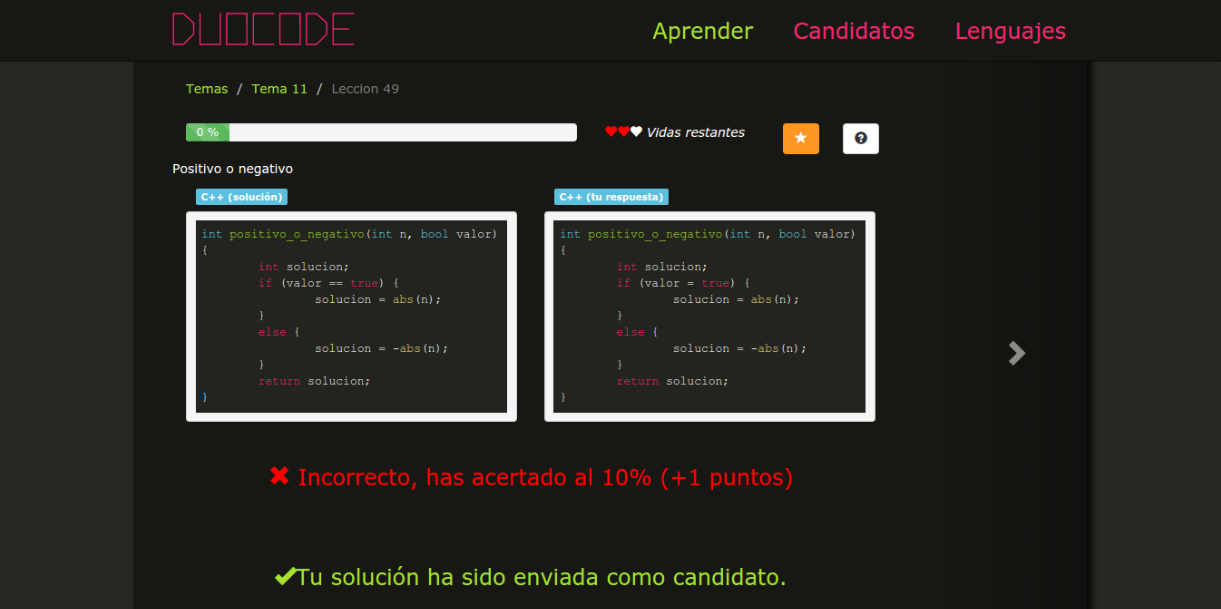
\includegraphics[scale=0.45]{images/enviarCandidato}}
\end{center}
\end{figure}

\end{itemize}

Hay dos posibilidades de acabar las lecciones:

\begin{itemize}

\item[•]Sin vidas: Una lección puede acabar si se acaban los corazones de los que dispone el usuario, es decir, si falla tres veces. Se muestra un botón mediante el cual el usuario puede volver a intentar la misma lección.

\begin{figure}[H]
\begin{center}
\makebox[\textwidth]{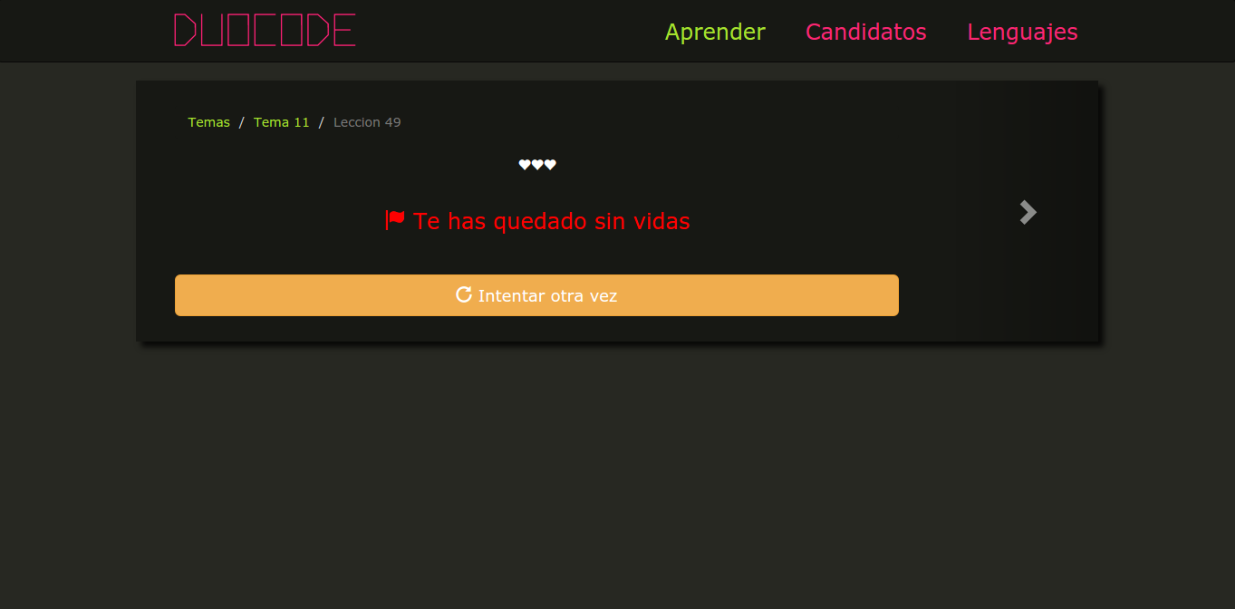
\includegraphics[scale=0.45]{images/sinVidas}}
\end{center}
\end{figure}

\item[•]Lección completada: Al acabar la lección con vidas, ésta se da como superada y se da la opción de compartir en Facebook el resultado. A partir de aquí podemos volver a las lecciones para seguir aprendiendo.

\begin{figure}[H]
\begin{center}
\makebox[\textwidth]{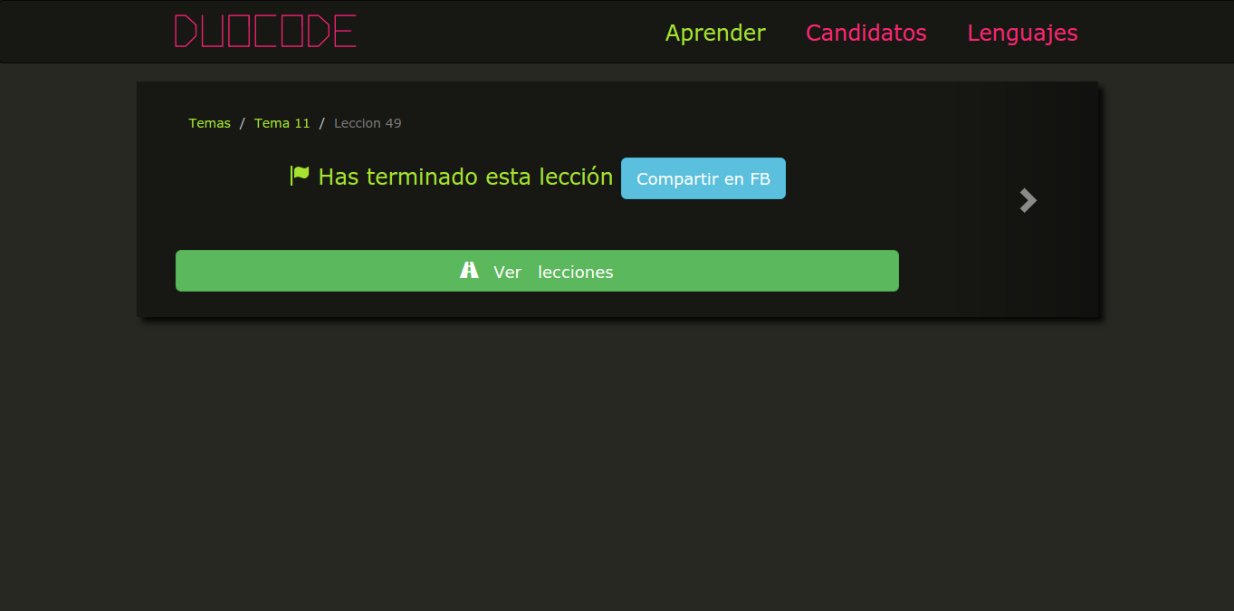
\includegraphics[scale=0.45]{images/leccionCompletada}}
\end{center}
\end{figure}

\begin{figure}[H]
\begin{center}
\makebox[\textwidth]{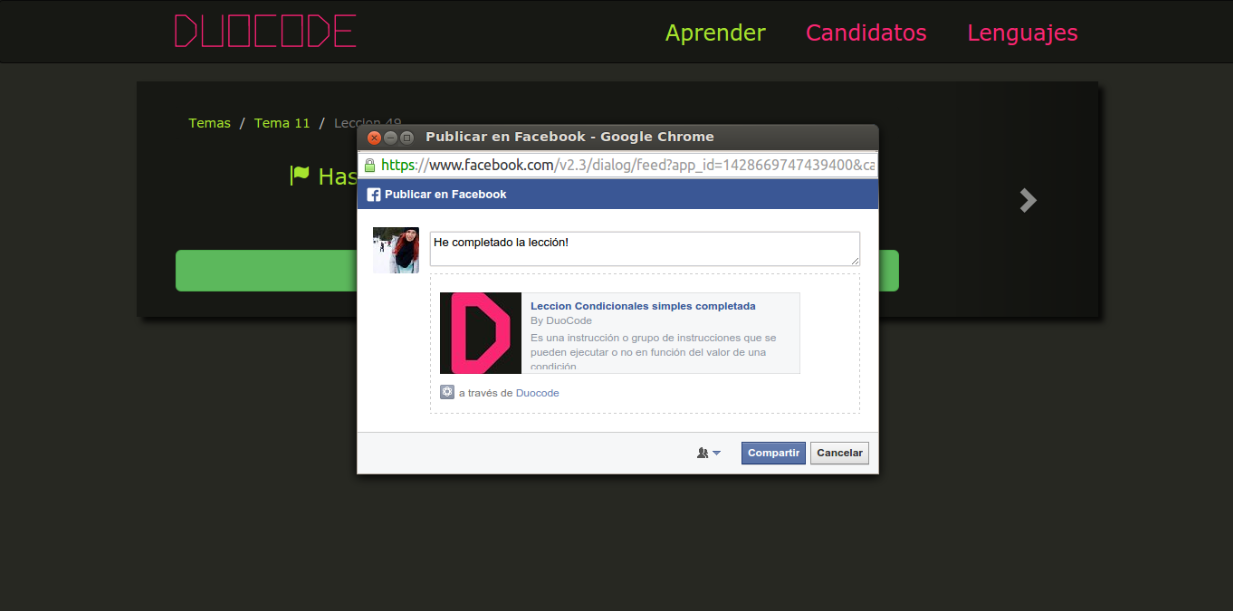
\includegraphics[scale=0.45]{images/compartirFB}}
\end{center}
\end{figure}

\end{itemize}

\subsection{Mis favoritos}

Desde la información de usuario se puede acceder a los favoritos del usuario. De cada ejercicio se muestra su título, los lenguajes que estaban seleccionados al marcar el ejercicio como favorito y un botón que al seleccionarlo muestra los códigos de origen y destino y la opción de desmarcarlo como favorito.

\begin{figure}[H]
\begin{center}
\makebox[\textwidth]{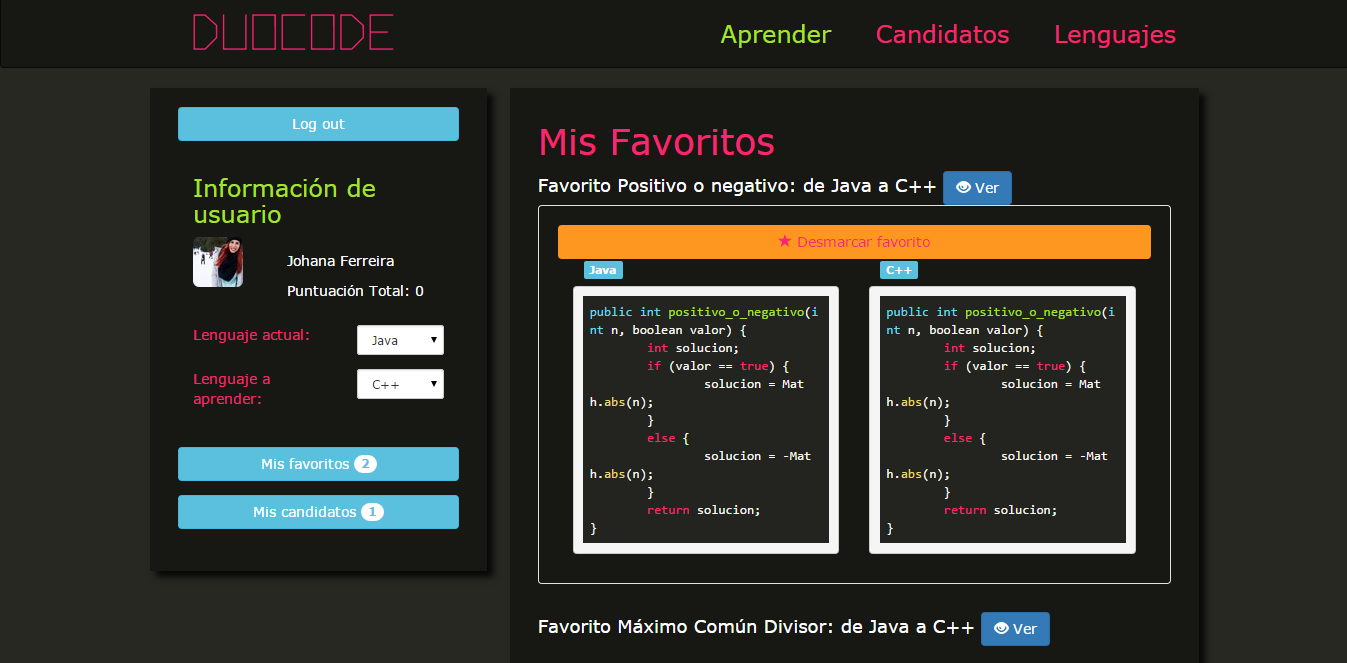
\includegraphics[scale=0.4]{images/favoritos}}
\end{center}
\end{figure}

\subsection{Mis candidatos}

Desde la información de usuario se puede acceder a los candidatos del usuario. De cada ejercicio se muestra su título, los lenguajes que estaban seleccionados al enviar el ejercicio como candidato y un botón que al seleccionarlo muestra el código del enunciado, la solución propuesta por el usuario y la opción de eliminar dicho candidato. Si el candidato ha sido aceptado o rechazado se indica en la parte superior.

\begin{figure}[H]
\begin{center}
\makebox[\textwidth]{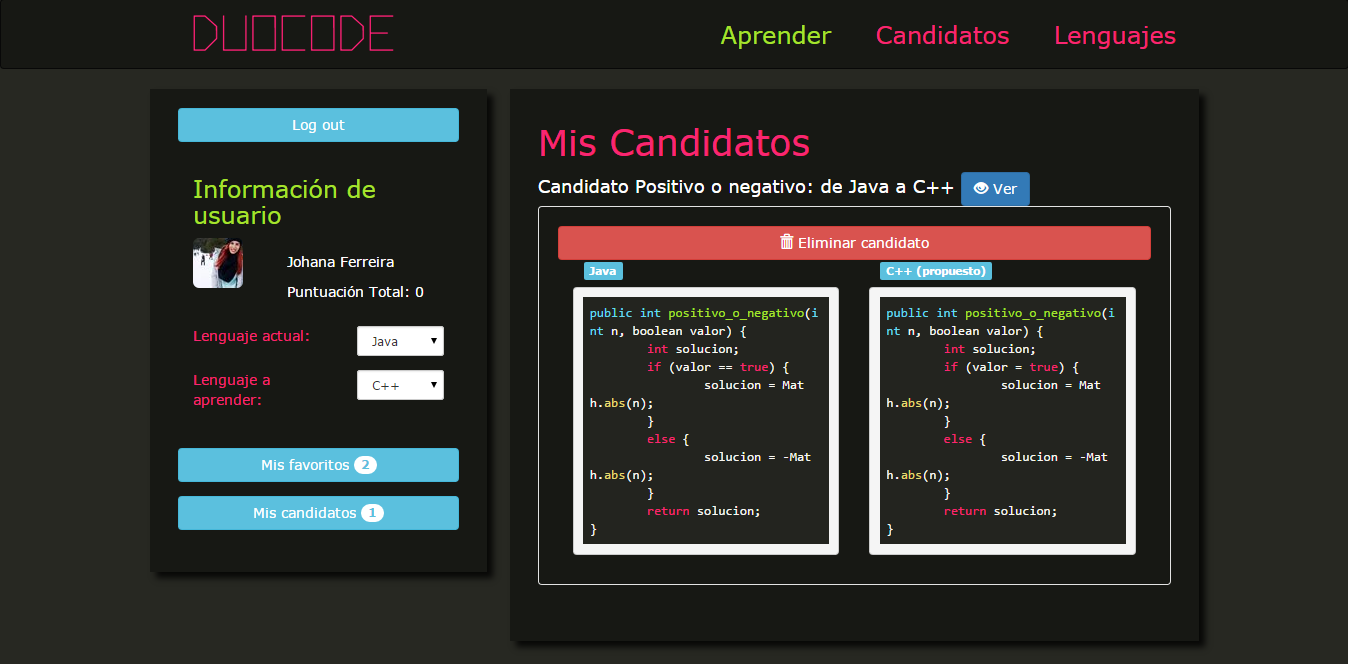
\includegraphics[scale=0.4]{images/misCandidatos}}
\end{center}
\end{figure}

\subsection{Candidatos}

Desde la barra de navegación tenemos acceso al apartado ``Candidatos'' en el cual se muestran los candidatos propuestos por los demás usuarios. De cada uno se muestra una barra con la cantidad de votos positivos y negativos que ha recibido, el nombre del ejercicio, el código del enunciado, el código propuesto a evaluación y dos botones en los que se puede votar si se está de acuerdo o no.

\begin{figure}[H]
\begin{center}
\makebox[\textwidth]{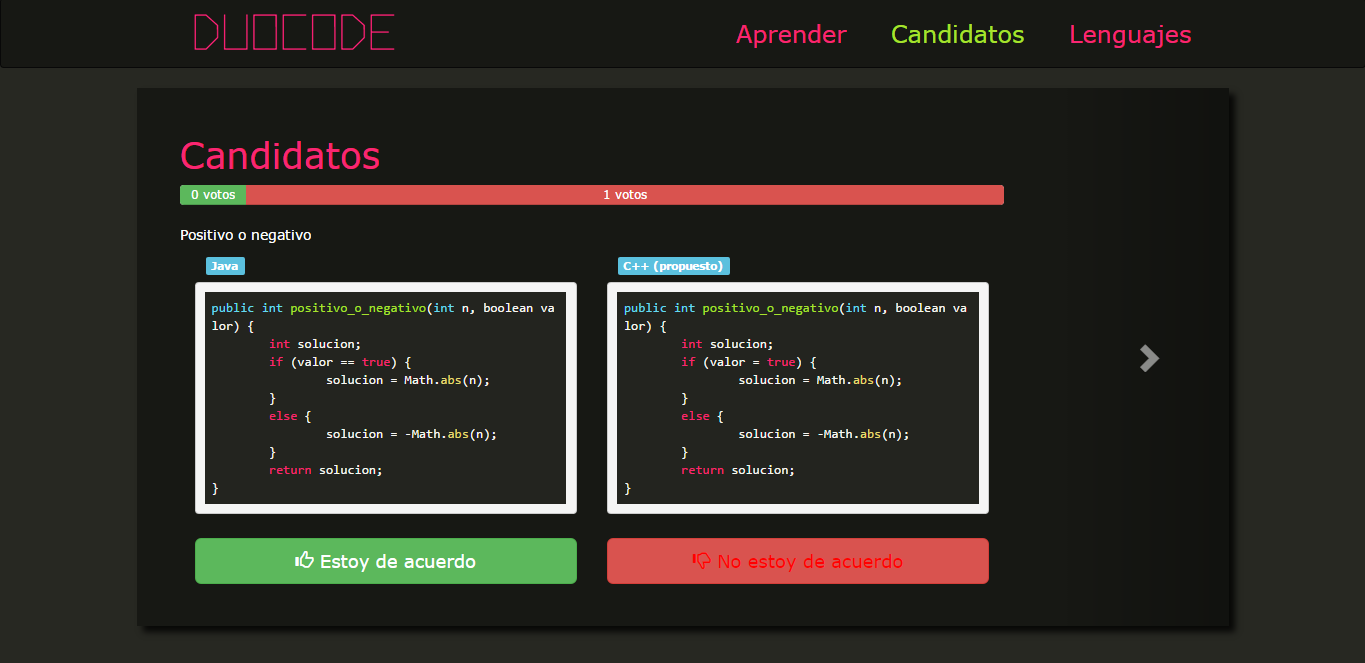
\includegraphics[scale=0.4]{images/candidatos}}
\end{center}
\end{figure}

Además, si el usuario es administrador se muestran otros dos botones adicionales mediante los cuales se acepta o rechaza un candidato definitivamente. Si se acepta pasa a ser solución válida del ejercicio, si se rechaza se elimina. En cualquiera de los casos ya no se encontrará en la lista de candidatos a evaluar.

\begin{figure}[H]
\begin{center}
\makebox[\textwidth]{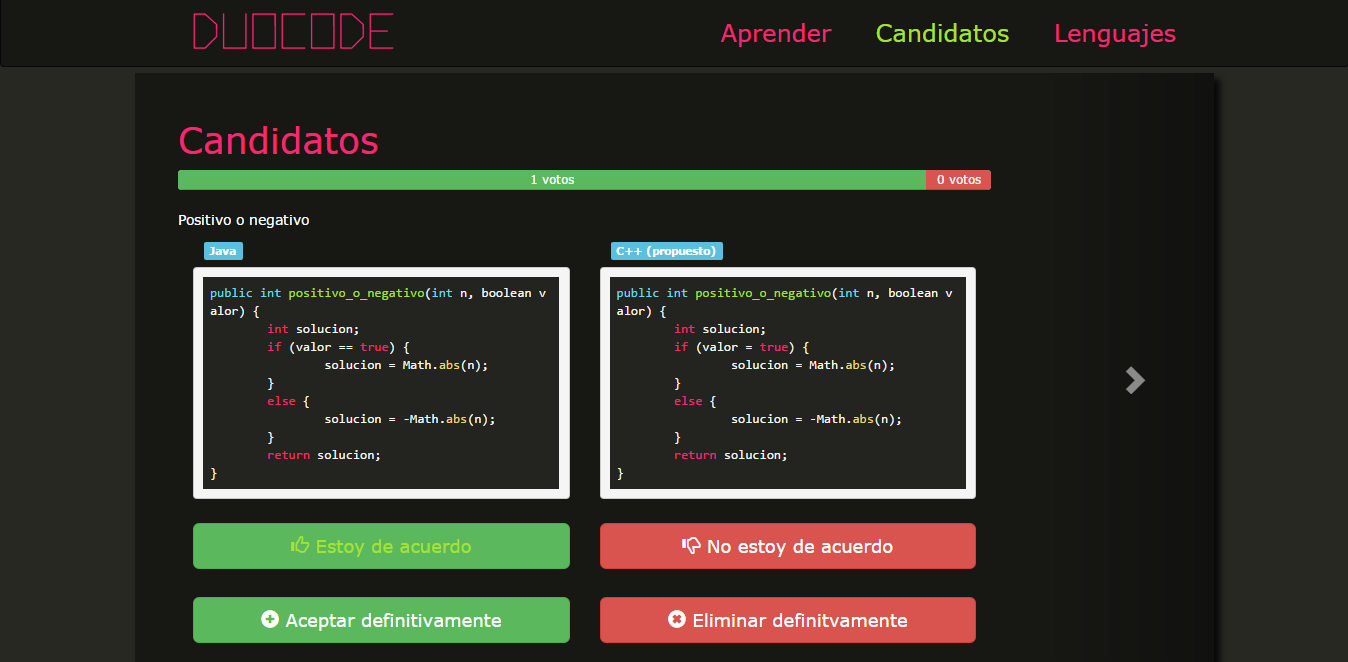
\includegraphics[scale=0.4]{images/candidatosAdmin}}
\end{center}
\end{figure}

Si ya se han evaluado todos los candidatos existentes se muestra un mensaje al usuario informándole de ello y un botón que le dirige a los temas para que siga aprendiendo.

\begin{figure}[H]
\begin{center}
\makebox[\textwidth]{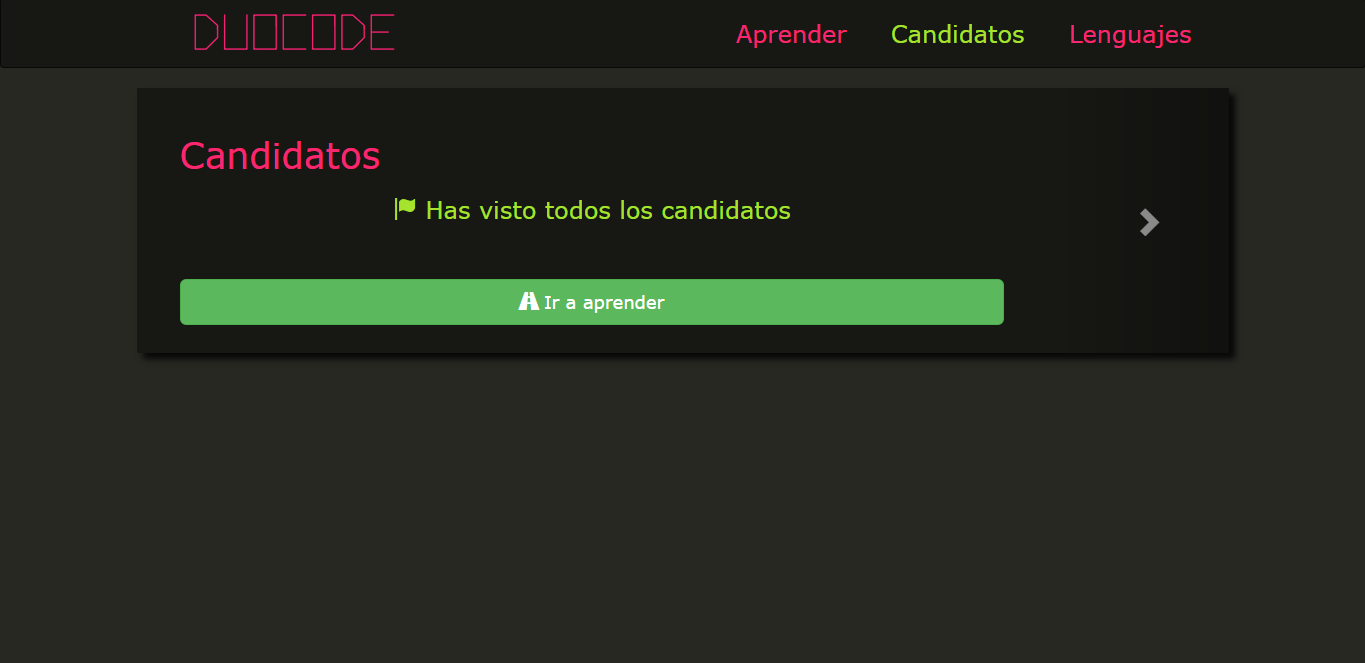
\includegraphics[scale=0.4]{images/sinCand}}
\end{center}
\end{figure}